\documentclass[12pt]{amsart}
% The srcltx package helps with inverse dvi search
%\usepackage{srcltx}

% This package has an easy way to set the margins
\usepackage[paper=letterpaper]{geometry}
\geometry{top=1in,left=1in,right=1in,bottom=1in,headheight=14pt}

% These packages include nice commands from AMS-LaTeX
\usepackage{algorithm}
\usepackage[noend]{algpseudocode}
%\usepackage[noend]{algpseudocode}
\usepackage{amssymb,amsmath,amsthm}
\usepackage{bm}
\usepackage{booktabs}
\usepackage{cancel}
\usepackage{caption}
\usepackage{changepage}
\usepackage{color}
\usepackage{comment}
\usepackage{empheq}
\usepackage[shortlabels]{enumitem}
\usepackage[mathscr]{euscript}
\usepackage{float}
\usepackage{graphicx}
\usepackage{hyperref}
%\usepackage[linktoc=none]{hyperref}
\usepackage{listings}
\usepackage{lscape}
\usepackage{multimedia}
\usepackage{setspace}
\usepackage{subfig}
\usepackage{tabularx}
\usepackage{textcomp}
\usepackage{tikz}
\usetikzlibrary{patterns}
\usetikzlibrary{scopes}
\usetikzlibrary{decorations.pathmorphing}
\usetikzlibrary{shapes,backgrounds, arrows}
\usepackage{xcolor}

%This package helps make nice headers
\usepackage{fancyhdr}
\pagestyle{fancy}
\lhead{\textsf{Note}}
\chead{\textsf{Jared McBride}}
\rhead{\textsf{\today}}
\renewcommand{\headrulewidth}{1pt}

% Make the space between lines slightly more
% generous than normal single spacing, but compensate
% so that the spacing between rows of matrices still
% looks normal.  Note that 1.1=1/.9090909...
\renewcommand{\baselinestretch}{1.1}
\renewcommand{\arraystretch}{.9090909}

\renewcommand{\and}{\qquad\text{and}\qquad}
\newcommand{\ds}{\displaystyle}

\DeclareMathOperator*{\argmax}{argmax}
\DeclareMathOperator*{\argmin}{argmin}

\newcommand\Fontvi{\fontsize{8}{7.2}\selectfont}
\newcommand{\vs}{\vspace{2 cm}}
\newcommand{\E}{\mathbb{E}}
\newcommand{\p}{\mathbb{P}}
\newcommand{\T}{\mathbb{T}}
\newcommand{\R}{\mathbb{R}}
\newcommand{\C}{\mathbb{C}}
\newcommand{\Q}{\mathbb{Q}}
\newcommand{\Z}{\mathbb{Z}}
\newcommand{\N}{\mathbb{N}}
\newcommand{\F}{\mathscr{F}}
\newcommand{\scrE}{\mathscr{E}}
\newcommand{\spa}{\text{span}}
\newcommand{\rref}{\mathrm{rref}}

\newcommand{\X}{\mathfrak{X}}
\newcommand{\ssX}{\bm{\textsf{X}}}
\newcommand{\ssx}{\bm{\textsf{x}}}
\newcommand{\fS}{\mathfrak{S}}
\newcommand{\fC}{\mathfrak{C}}

\renewcommand{\b}[1]{{\color{blue} #1}}
\usepackage[T1]{fontenc}
\usepackage{beramono}
\usepackage{listings}

\renewcommand{\and}{\qquad\text{and}\qquad }

\renewcommand{\P}{\mathbb{P}}
\newcommand{\cov}{\mathrm{cov}}
\newcommand{\var}{\mathrm{var}}
\newcommand{\abox}[1]
{
	\begin{center}
		\fbox{$\displaystyle #1$}
	\end{center}
}
%%
%% Julia definition (c) 2014 Jubobs
%%
\lstdefinelanguage{Julia}%
{morekeywords={abstract,break,case,catch,const,continue,do,else,elseif,end,export,false,for,function,immutable,import,importall,if,in,macro,module,otherwise,quote,return,switch,true,try,type,typealias,using,while},%
	sensitive=true,%
	alsoother={$},%
	morecomment=[l]\#,%
	morecomment=[n]{\#=}{=\#},%
	morestring=[s]{"}{"},%
	morestring=[m]{'}{'},%
}[keywords,comments,strings]%

\lstset{%
	language         = Julia,
	basicstyle       = \ttfamily,
	keywordstyle     = \bfseries\color{blue},
	stringstyle      = \color{magenta},
	commentstyle     = \color{olive},
	showstringspaces = false,
}

\newtheorem{theorem}{Theorem}
\newtheorem{lemma}{Lemma}
\newtheorem*{lem}{Lemma}

\title{Numerical Spectral Factorization by Kalman Recursion}
\author{Jared A. McBride}
\date{\today}
%
%\doublespacing

\begin{document}
	
\begin{abstract}
	In this note I describe a method presented by Kailath et al. in \cite{sayed2001} and \cite{kailath2000} for finding a spectral factor of the $z$-spectrum of a (wide-sense stationary) stochastic process under certain conditions. The method employs a version of Kalman filtering. As such I begin with a summary of relevant results from Kalman filtering. With those results in hand I present the method for finding spectral factors and conclude with examples.
\end{abstract}

\maketitle
\tableofcontents

\section{Introduction}

Given a wide-sense stationary (WSS) stochastic process $X = \big(X_n, n = 0, 1, \dots\big)$ it's $z$-spectrum $S_X(z)$ is defined by
$$S_X(z) = \sum_{n=-\infty}^\infty C_X[n]z^{-n},$$
where $C_X[n] = \E X_nX_0^*$ is the autocovariance sequence of the process $X$\footnote{
	A note on notation: the superscript $*$ denotes the complex conjugate transpose (Hermitian transpose) operator for matrices and just the complex conjugate for real or complex numbers. The superscripts $-*$ together is an abbreviation for the complex conjugate of the multiplicative inverse, i.e. $$z^{-*} = \frac{1}{z^*}.$$
}.
So that $S_X(z)$ is also the $z$-transform of the autocovariance sequence. This function is real-valued on the unit circle since, $C_X[-n] = C_X^*[n]$, and by the Wiener-Khinchin theorem, it is, in fact, nonnegative definite on the unit circle\footnote{
	Though what follows holds for scalar processes it also holds for vector valued processes. As such, I assume the vector case. Meaning, the covariance sequence is a sequence of square $d\times d$-matrices, where $d$ is the dimension of $X_0$.}.
Spectral factorization refers to a particular factorization in which 
$$S_X(z) = L(z)L^*(z^{-*})$$
where $L(z)$ is \emph{minimum phase}, meaning both $L(z)$ and $L^{-1}(z) = 1/L(z)$ are analytic on and outside the unit circle. The function $L$ will be referred to as a spectral factor of $S_X$. This factorization is not unique since for any spectral factor of $S_X$, right-multiplication by a unitary matrix produces another spectral factor of $S_X$. 

In this note I describe a method, presented by Kailath et al. in \cite{sayed2001} and \cite[p.~336]{kailath2000}, for finding a spectral factor under certain conditions. The method employs a version of Kalman filtering, more specifically the Kalman recursion for finding the innovations process for a process with a finite, linear state-space model. The innovations for such a process will be defined below. Section \ref{sec: Kalman} provides a summary of relevant results from Kalman filtering, together with some intuition relevant to the present context. With those results in hand, Section \ref{sec: Factor} presents the method for finding spectral factors. Then, in Section \ref{sec: Example} are examples.  

\section{Kalman Filtering}
\label{sec: Kalman}

The purpose of this section is to provide information from Kalman filtering theory that is pertinent to the development of the factorization algorithm to be discussed. To that end, the \textit{summum bonum} of the section is the computation of a modeling filter for a given process. The associated whitening filter also bears significance in this work and will be briefly treated. I begin by introducing the mathematical tools that I will be using, the inner product, norm, and the concept of linear least-mean-squares estimate appropriate to the context. A result is then provided that is important to the discussion of the Kalman filter. We then develop the Kalman filter in some generality and apply it to the time-invariant state-space process. We then add the assumption of stationarity and conclude the section with a theorem for a modeling filter of a given time-invariant (finite) state-space process that is stationary.




\subsection{Mathematical tools and context}

Suppose we have a (discrete-time) stochastic process
$X = \big(X_i,\; i =  0,1,2,\dots\big)$\footnote{
	From here till Section \ref{sec: Kalman stationary} $X$ need not be WSS.
} 
with a finite state-space representation of the following form:
\begin{subequations}
	\label{equ: ss}
	\begin{empheq}[left=\empheqlbrace]{align}
	\label{equ: ss State}\theta_{i+1} &= F_i\theta_i + G_iu_i \\
	\label{equ: ss Obs}X_i &= H_i\theta_i + v_i
	\end{empheq}
	where $F_i \in C^{m\times m},$ $G_i \in C^{m\times p},$ and $H_i \in C^{d\times m}$ are known matrices, and $u=(u_i)$, $v=(v_i)$, and $\theta_0$ are random variables with the following property\footnote{
		Throughout the note $$\delta_{ij} = \begin{cases} 1 &\text{if }i = j\\ 0 &\text{if }i \ne j.\end{cases}$$
	}
	\begin{equation}
	\E\begin{pmatrix} \theta_0 \\u_i \\ v_i \end{pmatrix}
	\begin{pmatrix} \theta_0 \\u_j \\ v_j\\1 \end{pmatrix}^*
	=\begin{pmatrix}
	\Pi_0 & 0                & 0              & 0 \\
	0     & Q_i\delta_{ij}   & S_i\delta_{ij} & 0 \\
	0     & S^*_i\delta_{ij} & R_i\delta_{ij} & 0
	\end{pmatrix}
	\label{equ: cond}
	\end{equation}
\end{subequations}

In the context here, I think of $X$ as a given series of\textit{ observations}, they are directly measurable, and $\theta = \big(\theta_i,\; i = 0,1,2,\dots\big)$ is the \textit{state} of the modeled process (usually not directly measurable). Both of these series are sequences of random variables, along with $u$ and $v$. The matrices $F_i$, $G_i$, $H_i$, $\Pi_0$, $Q_i$, $S_i$ and $R_i$ are deterministic for all $i$. 

Now, in the sequel there will be much discussion on  linear least-mean-square estimators (LMSEs). 
A nice thing about LMSEs is that there is an orthogonality principle, namely the estimator error is orthogonal to the predictor\footnote{
	The predictor refers to the random variable with respect to which the estimator is a linear combination. In our case this will exclusively be the observations, $X_i$}. 
What follows also affords such a principle. However, there is no Hilbert space that comfortably houses this theory. So, I will build up the context here. 

The context requires the consideration of vectors of more than one size, since the observations and the state need not be the same dimension. Since it is possible to write solutions to the problems I consider in terms of covariance information a natural ``inner product'' may be defined by
\begin{equation}
\langle x,y \rangle = \E xy^*\qquad \text{for all }x\in \C^d,y\in \C^m, \qquad d,m \in \N,
\label{def: inner p}
\end{equation}
So, that $\langle x,x \rangle \in \C^{d\times d}$ is the covariance of $x$ and $\langle x,y \rangle \in \C^{d\times m}$ is the cross covariance of $x$ and $y$. I use the notation $x \perp y$ if $x$ and $y$ are uncorrelated, meaning $\langle x,y \rangle = 0 \in \C^{d\times m}$.  

Because this inner product\footnote{
	If its arguments are restricted to the same linear space, it can be shown that $\langle \cdot, \cdot\rangle$ satisfies the axioms of an inner product, provided positivity is replaced with positive definiteness}
is matrix-valued, rather than adding structure to a linear space with a scalar \emph{field} the underlining space must be a module, with a \emph{ring} of (square) matrix-valued scalars. Because we are using linear combinations of variables of one dimension to estimate variables of a possibly different dimension, the natural choice of scalars are matrices of the appropriate size. This is an important point and leads me to this notation.
Let $$\text{span}_d\{y_i,\;i=0,1,\dots,N\} := \left\{\sum_{i=0}^N A_iy_i ~\bigg|~ y_i\in \C^{m_i},A_i \in \C^{d\times m_i},\quad i=0,1,\dots,N\right\}$$
I would like us to think of the span as possibly set in a different space from the arguments.

There is a norm 
\begin{equation}
\|x\|=\sqrt{\langle x,x \rangle}
\label{def: norm}
\end{equation} associated with this inner product, defined in the usual way, using the unique (Hermitian) positive-semidefinite square root of the Hermitian positive-semidefinite matrix $\langle x,x \rangle$.   


I have just introduced the context and notation with which we will be describing spectral factorization. 

\subsection{the Kalman filter}
Now, the Kalman filter allows us to find, for some $i>0$, the linear LMSE of the state $\theta_{i+1}$ given all preceding observations $X_j$ for $j = 0,1,2,\dots, i$. 
This quantity I will denote by $\hat{\theta}_{i+1|i}$. Since in this note I will only be concerned with linear LMSEs given the $X_j$'s, the subscript $\cdot_{|i}$ will denote linear estimators with respect to and conditioned on all $X_j$ for $j \le i$. 
Consistent with this convention, when I write $\hat{X}_{i|i-1}$ I mean the linear LMSE of $X_i$ given $X_j$ for $j < i$. 

For the stake of rigor and completeness I have provided a lemma which describes the orthogonality principle in this context. For the sake of brevity I have placed the proof in Appendix \ref{app: Ortho proof}.

\begin{lemma}
	\label{lem: otho p}
	Given the inner product defined under (\ref{def: inner p}) and the norm induced by it, under (\ref{def: norm}), let $x\in C^d$ and $y_i \in \C^m$ for $i=0,\dots,N$ be random variables. If $\hat x\in \text{span}_d\{y_i,\;i=0,1\dots,N\}$ is chosen such that \begin{equation}
	(x-\hat x) \perp y_i \qquad\text{\emph{for}}\qquad i=0,1,\dots,N,
	\end{equation}
	then $\hat x$ is the linear LMSE for $x$ given $\{y_i,\;i=0,\dots,N\}$, meaning
	$$\E(x-\hat x)(x-\hat x)^* = \|x-\hat x\|^2 = \inf_{x'\in \text{\emph{span}}_d\{y_i,\;\forall i\}} \|x-x'\|^2.$$
\end{lemma}


\subsection{Kalman filter recursions for the innovations}

Now, with these ideas in mind, we seek a LMSE of $\theta_{i+1}$ restricted to a linear (matrix-valued coefficient) combination of observations, $\{X_j,\;j < i\}$. This means we seek $\hat\theta_{i+1|i}$ such that,
\begin{align}
	\hat\theta_{i+1|i} &\in\mathcal{L}_{d,i} := \text{span}_d\{X_i,\;i=0,1,\dots,N\}\\
	\label{equ: cond proj}\hat\theta_{i+1|i} &= \displaystyle\argmin_{\hat\theta \in \mathcal{L}_{d,i}}\|\theta_{i+1} - \hat\theta\|^2.
\end{align}
Borrowing from Hilbert space theory, we consider building an orthogonal basis for the space $\mathcal{L}_{m,i} := \text{span}_m\{X_i,\;i=0,1,\dots,N\}$ (recall $X_0 \in \C^m$), $\{e_j,\;j = 1,2,\dots,i\}$. Then project $\theta_{i+1|i}$ on to $\mathcal{L}_{d,i}$ by the formula 
\begin{equation}
\hat{\theta}_{i|k} = \sum_{j=0}^k \langle \theta_{i}, e_j \rangle R^{-1}_{e,j} e_j\qquad k<i
\label{equ: projection}
\end{equation}
where $R_{e,i} = \langle e_i, e_i \rangle$. We are not in a Hilbert space, so the claim that the estimator under (\ref{equ: projection}) satisfies (\ref{equ: cond proj}) will need to be verified. To that end, let us, first, build this orthogonal set $\{e_j,\;j = 1,2,\dots,i\}$. I proceed in a way similar to the Gram-Schmidt process, but without normalizing. Put
$e_0 = X_0$ and proceed for $i>0$ iteratively by
\begin{equation}
e_i = X_i - \sum_{j=0}^{i-1} \langle X_i, e_j \rangle R_{e,j}^{-1}e_j.
\end{equation}
Certainly, $\text{span}_{m}\{e_j,\;j=0,1,\dots,i\} = \mathcal{L}_{m,i}$. I will show orthogonality of the set $\{e_j,\;j = 1,2,\dots,i\}$ explicitly since matrix inner products are not very common. I proceed by induction. Observe that for $i=1$
\begin{align*}
\langle e_0,e_1 \rangle &= \langle e_0,X_1 - \langle X_1,e_0\rangle R_{e,0}^{-1} e_0 \rangle\\
&=\langle e_0,X_1\rangle - \langle e_0, \langle X_1,e_0\rangle R_{e,0}^{-1} e_0 \rangle\\
&=\langle e_0,X_1\rangle - \langle e_0,e_0 \rangle R_{e,0}^{-1} \langle e_0,X_1 \rangle = 0.
\end{align*}
Here the facts that $R_{e,0}$ is hermitian and that $\langle X_1,e_0\rangle^* = \langle e_0,X_1\rangle$ were used. Now, suppose for any $i<k$ and $j<i$ that $\langle e_j,e_i \rangle = 0$, and observe that for $j<k$
\begin{align*}
\langle e_j,e_k \rangle &= \left\langle e_j,X_k - \sum_{l=0}^{k-1}\langle X_k,e_l\rangle R_{e,l}^{-1} e_l \right\rangle\\
&= \langle e_j,X_k\rangle - \sum_{l=0}^{k-1} \langle e_j,\langle X_k,e_l\rangle R_{e,l}^{-1} e_l \rangle\\
&= \langle e_j,X_k\rangle - \sum_{l=0}^{k-1} \langle e_j,e_l \rangle R_{e,l}^{-1} \langle e_l,X_k\rangle \\
&= \langle e_j,X_k\rangle - \langle e_j,e_j \rangle R_{e,j}^{-1} \langle e_j,X_k\rangle = 0.
\end{align*}
And so, $\langle e_i,e_j \rangle = \R_{e,i}\delta_{ij}$ for all $i,j \ge 0$. A consequence of this orthogonality results together with Lemma \ref{lem: otho p} is the more intuitively useful equation
$$e_i = X_i - \hat{X}_{i|i-1}\quad \text{for }i>0.$$
For this reason, the process $e = (e_i,\; i= 0, 1, 2,\dots)$ is commonly referred to as the \textit{innovations} associated with $X$. 
And now I can prove equation (\ref{equ: projection}). Using Lemma \ref{lem: otho p} we need only show $$\left(\theta_{i} - \sum_{l=0}^k \langle \theta_{i}, e_l \rangle R^{-1}_{e,l} e_l\right)\perp e_j \qquad \text{for} j = 0, 1, \dots, k.$$
To that end consider the following for $0 < j \le k<i$
\begin{align*}
\left\langle e_j, \theta_{i} - \sum_{l=0}^k \langle \theta_{i}, e_l \rangle R^{-1}_{e,l} e_l\right\rangle &= \langle e_j, \theta_i \rangle - \sum_{l=0}^k \left\langle e_j,\langle \theta_{i}, e_l \rangle R^{-1}_{e,l} e_l\right\rangle\\
&= \langle e_j, \theta_i \rangle - \sum_{l=0}^k \left\langle e_j,e_l\right\rangle R^{-1}_{e,l}\langle  e_l, \theta_{i}\rangle  \\
&= \langle e_j, \theta_i \rangle - \left\langle e_j,e_j\right\rangle R^{-1}_{e,j}\langle  e_l, \theta_{i}\rangle = 0.
\end{align*}
Thus we verify equation (\ref{equ: projection}) by Lemma \ref{lem: otho p}.

There are other orthogonality relations I would like to highlight. First noting that $\theta_i \in \text{span}_m\{\theta_0, u_j,\; j<i\}$, then by use of (\ref{equ: ss Obs}) and the definition of $e_i$ one can show the following.
\begin{subequations}
	\label{equ: inner p}
\begin{align}
\langle \theta_i, u_j \rangle = 0 &\and \langle \theta_i, v_j \rangle = 0 \qquad\;\;\;\text{for}\qquad i\le j;\\
\label{equ: inner p b}\langle X_i, u_j \rangle = 0 &\and \langle X_i, v_j \rangle = 0 \qquad\;\;\text{for}\qquad i < j;\\
\langle X_i, u_j \rangle = S^*_i &\and \langle X_i, v_j \rangle = R_i \qquad\text{for}\qquad i = j;\\ 
\langle e_i, u_j \rangle = 0 &\and \langle e_i, v_j \rangle = 0 \qquad\;\;\;\text{for}\qquad i < j;\\
\label{equ: inner p e} \langle e_i, u_j \rangle = S^*_i &\and \langle e_i, v_j \rangle = R_i \qquad\;\text{for}\qquad i = j.
\end{align}
\end{subequations}

Now, Kalman developed a recursion to cheaply find the innovations process associated with the observations, which we will derive here.
I like the way Kailath put it, ``It turns out that the recursive construction of the innovations combines nicely with the recursive evolution of the state variables to give a recursion for the innovations...''\cite[p.~312]{kailath2000}.

We seek a recursion for $\{e_j\}$ but start with finding a recursion for $\hat{\theta}_{i|i-1}$ using (\ref{equ: projection}),
\begin{align*}
\hat{\theta}_{i+1|i} &= \sum_{j=0}^i \langle \theta_{i+1}, e_j \rangle R^{-1}_{e,j} e_j\\
&= \left(\sum_{j=0}^{i-1} \langle \theta_{i+1}, e_j \rangle R^{-1}_{e,j} e_j\right) + \langle \theta_{i+1}, e_i \rangle R^{-1}_{e,i} e_i\\
& = \hat{\theta}_{i+1|i-1} + \langle \theta_{i+1}, e_i \rangle R^{-1}_{e,i} e_i.
\end{align*}
The first term of the last line undermines the recursion in $\hat{\theta}_{i|i-1}$; however, we can remedy this by projecting equation (\ref{equ: ss State}) on $\mathcal{L}_{d,i-1}$ to get
$$\hat{\theta}_{i+1|i-1} = F_i\hat{\theta}_{i|i-1} +G_i\hat{u}_{i|i-1} = F_i\hat{\theta}_{i|i-1} + 0$$
by (\ref{equ: inner p b}). This provides
$$\hat{\theta}_{i+1|i} = F_i\hat{\theta}_{i|i-1} + \langle \theta_{i+1}, e_i \rangle R^{-1}_{e,i} e_i$$
The next thing to do is to make sure we can compute $e_i$ from the $\hat{\theta}_{i|i-1}$'s. If we project equation (\ref{equ: ss Obs}) on $\mathcal{L}_{m,i-1}$ then 
\begin{equation}
\hat{X}_{i|i-1} = H_i\hat{\theta}_{i|i-1} + \hat{v}_{i|i-1} = H_i\hat{\theta}_{i|i-1} + 0\label{equ: X hat}
\end{equation}
also by (\ref{equ: inner p b}). So, that
$$e_i = X_i - \hat{X}_{i|i-1} = X_i - H_i\hat{\theta}_{i|i-1}.$$ 
From this point I will use the abbreviated notation $\hat{\theta}_i = \hat{\theta}_{i|i-1}$.

Putting this together, we get a recursion for the innovations
\begin{subequations}
	\begin{empheq}[left=\empheqlbrace]{align}
		\label{equ: theta hat} \hat{\theta}_{i+1} &= F_i\hat{\theta}_{i} + K_ie_i, \quad \hat{\theta}_0 = 0\\
		\label{equ: innov} e_i &= X_i - H_i \hat{\theta}_{i}.
	\end{empheq}
\end{subequations}
where $K_i = \langle \theta_{i+1}, e_i \rangle R^{-1}_{e,i}$. 

Here then is the recursion we sought, which recursively generates the innovations associated with the process $X$. 
It turns out that for spectral factorization we do not need the innovations themselves; we only need the $K_i$ and $R_{e,i}$ and would therefore expect savings if these could be computed independently from the observations. In fact this is possible and I will demonstrate how this may be accomplished.

Let $\tilde{\theta}_i = \theta_i - \hat{\theta}_{i}$ and $P_{i} = \langle \tilde{\theta}_{i},\tilde{\theta}_{i} \rangle$. This quantity is very useful in formulating an observation-free recursion. It is easy to see by subtracting (\ref{equ: X hat}) from (\ref{equ: ss Obs}) that $e_i = H_i\tilde{\theta}_{i} - v_i$, and this is enough to put $R_{e,i}$ in terms of $P_i$.
Observe that because $\hat{\theta}_{i}\in \mathcal{L}_{d,i}$,  $\hat{\theta}_{i}$ is orthogonal to $v_i$ by (\ref{equ: inner p b}). And this yields,
$$R_{e,i} = H_iP_iH^*_i + R_i.$$
To get $K_i$ in terms of only $P_i$ and $R_{e,i}$, we start with $K_i = \langle \theta_{i+1}, e_i \rangle R_{e,i}^{-1}$ and observe that by (\ref{equ: ss Obs}) $\langle \theta_{i+1}, e_i \rangle = F_i\langle \theta_{i}, e_i \rangle  + G_i\langle u_i, e_i \rangle$. Reflecting on both inner products in turn provides
\begin{align*}
\langle \theta_{i}, e_i \rangle &= \langle \theta_{i}, H\hat\theta_i - v_i \rangle\\
&= \langle \theta_{i}, \tilde{X}_i \rangle H^*_i - \langle \theta_{i}, v_i \rangle \\
&= \langle \hat\theta_{i} + \tilde\theta_i, \tilde\theta_i \rangle H^*_i + 0 \\
&= P_i H^*_i
\end{align*}
and $\langle u_{i}, e_i \rangle = S_i$, as we have seen in (\ref{equ: inner p e}). Substituting, we able to find that
$$K_i = (F_iP_iH_i^* + G_iS_i) R_{e,i}^{-1},$$
as desired.
Now, with $R_{e,i}$ and $K_i$ in place, a recursion for $P_i$ can be established by
combining equations (\ref{equ: ss State}) and (\ref{equ: theta hat}) and taking the covariance of both sides, a somewhat long calculation results in the recursion,
\begin{align}
\label{equ: DL} P_{i+1} &= F_iP_{i}F_i^* + G_iQ_iG_i^* - K_iR_{e,i}K^*_i,\qquad i\ge 0
\end{align}
which we initialize by $$P_{0} = \langle \hat{\theta}_{0}, \hat{\theta}_{0} \rangle = \langle \theta_0, \theta_0 \rangle = \Pi_0.$$ 


We have just found a system of recursions for the $K_i$ and $R_{e,i}$, which is independent of observations. It also provides a recursion for the error covariance of the state estimate (which is useful in its own right).  The discussion so far can be summarized into a theorem
\begin{theorem}
	\label{thm: innov}
	Consider the state-space model
	$$\left\{\begin{array}{ r l}
	\theta_{i+1} &= F_i\theta_i + G_iu_i \\
	X_i &= H_i\theta_i + v_i
	\end{array}\right. $$
	for $i\ge 0$, and satisfying (\ref{equ: cond}). The innovations process of $X$ can be recursively computed using the equations
	\begin{subequations}
		\label{equ: innovations}
		\begin{empheq}[left=\empheqlbrace]{align}
			e_i &= X_i - H_i\hat{\theta}_i, \qquad i \ge 0,\\
			\hat{\theta}_{i+1} &= F_i\hat{\theta}_i + K_{i}e_i,\qquad \hat{\theta}_0 = 0,
		\end{empheq}
	\end{subequations}
	where 
	\begin{subequations}
		\label{equ: Kal}
		\begin{align}
			\label{equ: Kal Pi}  P_{i+1} &= F_iP_{i}F_i^* + G_iQ_iG_i^* - K_iR_{e,i}K^*_i,\qquad P_0 = \Pi_0, \\
			\label{equ: Kal Rei} R_{e,i} &= H_i P_i H^*_i + R_i, \\
			\label{equ: Kal Ki}  K_i &= (F_i P_iH_i^* + G_iS_i) R_{e,i}^{-1}.
		\end{align}
	\end{subequations}
	Here, $P_i = \langle \tilde{\theta}_i,\tilde{\theta}_i \rangle$ where $\tilde{\theta}_i = \theta_i - \hat{\theta}_i$.
\end{theorem}

\subsection{The Stationary Case and the Modeling Filter}
\label{sec: Kalman stationary}

So far in this section, all we have assumed about $X$ is that it is a discrete-time stochastic process that has a finite state-space representation defined by (\ref{equ: ss}). But now it is time to assume conditions native to the problem at hand, which will be delineated shortly. These assumptions are afforded by the stationarity of the processes I work with.  The plan is to realize stationarity and adjust the innovations process so as to produce both stationary innovations and stationary state estimators.

Here are the further assumptions I impose on the process $X$, 
\begin{itemize}
	\item the state-space representation for $X$ is time-invariant, meaning, all the parameters are constant in time. So,
	$$F_i = F,\quad G_i=G, \quad H_i = H,\quad Q_i=Q, \quad S_i=S \quad\text{and}\quad R_i = R\qquad \text{for }i\ge 0$$
	additionally I impose that $F$ be stable (meaning its eigenvalues lie strictly in the unit circle) and $R$ be strictly positive-definite, $R>0$, also 
	\item $\theta_i$ is in  steady state, meaning $\Pi_i = \Pi$ for $i\ge 0$ where is $\Pi$ is the positive-semi-definite solution to the Lyapunov equation. 
	\begin{equation}
	\Pi = F\Pi F^* + GQG^*.
	\label{equ: state Lyapunov}
	\end{equation}
	 Since $F$ is stable this has a unique solution. 
\end{itemize}

A consequence of these assumptions in that $X$ is wide-sense stationary, and it's model can be written as 
\begin{subequations}
	\label{equ: ss ss}
	\begin{empheq}[left=\empheqlbrace]{align}
	\label{equ: ss ss State}\theta_{i+1} &= F\theta_i + Gu_i \\
	\label{equ: ss ss Obs}X_i &= H\theta_i + v_i
	\end{empheq}
	where
	\begin{equation}
	\E\begin{pmatrix} \theta_0 \\u_i \\ v_i \end{pmatrix}
	\begin{pmatrix} \theta_0 \\u_j \\ v_j\\1 \end{pmatrix}^*
	=\begin{pmatrix}
	\Pi & 0                & 0              & 0 \\
	0     & Q\delta_{ij}   & S\delta_{ij} & 0 \\
	0     & S^*\delta_{ij} & R\delta_{ij} & 0
	\end{pmatrix}
	\label{equ: cond ss}
	\end{equation}
\end{subequations}
It can be show by direct computation that the covariance function of $X$, $R_X(i-j)$, can be written as follows \cite[p.~267]{kailath2000}
\begin{equation}
R_X(i-j) = \begin{cases}
	HF^{i-j-1}N & i>j, \\
	R + H\Pi H^* & i = j, \\
	N^*(F^*)^{j-i-1}H^* & i < j,
\end{cases}
\label{equ: autocov X}
\end{equation}
where $N= F\Pi H^* + GS$.


Under these conditions we now apply Theorem \ref{thm: innov} and find that the innovations sequence associated with $X$ has the following state-space representation 
\begin{subequations}
	\label{equ: innovations stationary}
	\begin{align}
	e_i &= X_i - H\hat{\theta}_i, \qquad i \ge 0,\\
	\hat{\theta}_{i+1} &= F\hat{\theta}_{i} + K_{i}e_i,\qquad \hat{\theta}_0 = 0,	
	\end{align}
\end{subequations}
	where now
	\begin{subequations}
	\label{equ: Kal stationary}
	\begin{align}
	\label{equ: Kal stationary Pi}  P_{i+1} &= FP_{i}F^* + GQG^* - K_iR_{e,i}K^*_i,\qquad P_0 = \Pi \\
	\label{equ: Kal stationary Rei} R_{e,i} &= HP_iH^* + R \\
	\label{equ: Kal stationary Ki}  K_i &= (FP_iH^* + GS) R_{e,i}^{-1}
	\end{align}
\end{subequations}


Rearranging (\ref{equ: innovations stationary}) slightly we can write
\begin{subequations}
	\label{equ: model}
	\begin{empheq}[left=\empheqlbrace]{align}
		\hat{\theta}_{i+1} &= F \hat{\theta}_{i} + K_{i} e_i,\qquad \hat{\theta}_0 = 0,\\
		X_i &= H\hat{\theta}_i + e_i, \qquad i \ge 0.
	\end{empheq}
\end{subequations}
Which provides an alternative way of modeling the process $X$, this time driven by the innovations process $e$. Said differently (\ref{equ: model}) defines a system $\mathcal{L}$ which maps $e$ to $X$. The system $\mathcal{L}$ is sometimes referred to as a modeling filter since given the noise sequence $e$ it will recover $X$, exactly.

Observe that $\mathcal{L}$, clearly causal, is also causally invertable since by algebra we can write,
\begin{subequations}
	\label{equ: white}
	\begin{empheq}[left=\empheqlbrace]{align}
		\hat{\theta}_{i+1} &= (F - K H)\hat{\theta}_{i} + K_{i}X_i,\qquad \hat{\theta}_0 = 0,\\
		e_i &= - H\hat{\theta}_i + X_i, \qquad i \ge 0.
	\end{empheq}
\end{subequations}
This contrasts with the original model which took $(\theta_0, u, v)$ to $X$\footnote{
	One thing it has done was remove the additional input variable, the initial state, setting it to zero}, 
such is causal but not generally causally invertible. 

Now, what can be said about the output $\mathcal{L}w$, for $w = (w_i,\; i = 0, 1, 2, \dots)$ a noise sequence with $\langle w_i, w_j \rangle = R_{e,i}\delta_{ij}$? Is it a stationary process with the same $z$-spectrum as $X$? No, generally the output is not even stationary, since the model, found under (\ref{equ: model}), represents a time-variant system. This begs the question, does this model converge, in time, to a time-invariant model? It turns out that the system parameters $P_i$, $R_{e,i}$, and $K_i$ all converge as $i\rightarrow \infty$. Which suggests a time-invariant causal system that, when fed in a stationary input, will certainly produce a stationary output. A \textit{modeling filter} for $X$ is a causal, linear system which constructs the process $X$ by passing a white-noise process through the filter. This is what we are seeking.  

The convergence of $P_i$ has been well studied \cite[Sec.~14.5]{kailath2000} and there are many conditions one can check to ensure that the limit of the recursion converges to the stabilizing solution of the appropriate Ricatti equation necessary to provide the causal and casually invertible modeling filter, namely the discrete algebraic Riccati equation (DARE), given by
\begin{align}
P &= FPF^* + GQG^* - (FPH^* + GS)(HPH^* + R)^{-1}(HPF^* + S^*G^*)\\
 &= FPF^* + GQG^* - KR_eK^*
\label{equ: recatti equation}
\end{align}
Since this theory is more problem dependent I will defer the matter of convergence to when we have a specific problem. 


So, for now, assume that
$$\lim_{i\rightarrow \infty} P_i = P$$
So that $P$ in the unique solution to 
\begin{equation}
	P = FPF^* + GQG^* - KR_eK^*
	\label{equ: racatti}
\end{equation}
where $R_e = \lim R_{e,i} =  HPH+R$ and $K = \lim K_i =   (FPH^* + GS)R^{-1}_e$, and that $P$ is such that $F - KH$ is stable. Let us, then, consider the system $$L: w \mapsto Y $$ where $w = (w_i,\; i \ge -\infty)$ with $ \langle w_i,w_j \rangle = R_e\delta_{ij}$ and $Y = (Y_i,\; i \ge -\infty)$\footnote{Notice the slight-of-hand, we now start our processes in the remote past and have them be bilaterally infinite. This is to obviate the need for the state variable to be initialized as an input in order for them to have a variance that obeys the Lyapunov equation below for each finite time} given by 
\begin{subequations}
	\label{equ: modeling}
	\begin{empheq}[left=\empheqlbrace]{align}
		\eta_{i+1} &= F\eta_{i} + Kw_i,\qquad \eta_{-\infty} = 0\\
		Y_i &= H\eta_i+ w_i, \qquad i \ge -\infty.	
	\end{empheq}
Since $\eta_i$ was initialized in the remote past (independent of $w_i$) we have $\langle \eta_i, w_i \rangle = 0$ for $i> -\infty$ and $\langle \eta_i, \eta_i \rangle = \Sigma$ for $i> -\infty$
where 
\begin{align}
\Sigma =F\Sigma F^* +KR_eK^*.
\end{align}
\end{subequations}


We want to check that the autocovariance of $Y$ is the same as for $X$ which is given in (\ref{equ: autocov X}). This can be checked directly. For $i>0$
\begin{align*}
R_Y[i] &= \langle Y_i, Y_0 \rangle \\
	&= \langle H\eta_i+w_i, H\eta_0 + w_0 \rangle \\
	&= \langle HF\eta_{i-1}+HKw_{i-1} + w_i, H\eta_0 + w_0 \rangle \\
	&= \langle HF^2\eta_{i-2}+HFKw_{i-2} + HKw_{i-1} + w_i, H\eta_0 + w_0 \rangle \\
	&= \langle HF^i\eta_{0}+HF^{i-1}Kw_{0} + \dots + HFKw_{i-2} + HKw_{i-1} + w_i, H\eta_0 + w_0 \rangle \\
	&= \langle HF^i\eta_{0}, H\eta_0\rangle + \langle HF^{i-1}Kw_{0} + \dots + HFKw_{i-2} + HKw_{i-1} + w_i, H\eta_0 \rangle \\
	&\qquad +\langle HF^i\eta_{0}, w_0\rangle + \langle HF^{i-1}Kw_{0} + \dots + HFKw_{i-2} + HKw_{i-1} + w_i, w_0 \rangle\\
	&= HF^i\Sigma H^* + 0 + 0 + HF^{i-1}KR_e\\
	&= HF^i\Sigma H^* + HF^{i-1}(FPH^* + GS)\\
	&= HF^{i-1}\big(F(\Sigma + P)H^* + GS)\big),
\end{align*}
a similar calculation for $i<0$ yields
\begin{align*}
R_Y[i] = \big(F(\Sigma + P)H^* + GS)\big)^*(F^*)^{i-1}H^* = R^*_Y[-i],
\end{align*}
and for $i=0$
\begin{align*}
	 R_Y(0) &= \langle Y_0, Y_0 \rangle \\
	 &= \langle H\eta_0+w_0, H\eta_0 + w_0 \rangle \\
	 &= H\Sigma H^* + R_e \\
	 &= H\Sigma H^* + HPH^* + R\\
	 &= H(\Sigma + P)H^* + R
\end{align*}
Now what is $\Sigma + P$, by there definitions 
\begin{align*}
\Sigma + P &= F\Sigma F^* + KR_eK^* + FPF^* + GQG^* - KR_eK^*\\
&= F(\Sigma + P)F^* + GQG^*.
\end{align*}
Meaning that $\Sigma + P$ solves the same discrete Lyapunov equation that $\Pi$ solved in (\ref{equ: state Lyapunov}). We therefore conclude $$\Pi = \Sigma + P$$ and that 
\begin{equation}
R_Y[i] = \begin{cases}
HF^{i-1}N & i>0, \\
R + H\Pi H^* & i = 0, \\
N^*(F^*)^{-i-1}H^* & i < 0,
\end{cases} \qquad= R_X[i]
\label{equ: autocov Y}
\end{equation}
recalling that  $N= F\Pi H^* + GS$, as in equation (\ref{equ: autocov X}). 
The system $L$ maps \emph{any} white-noise sequence with variance $R_e$ to a stationary process with a given $z$-spectrum. This is what I refer to as a \emph{weak} modeling filter. 

Furthermore, observe that $L$ (given by (\ref{equ: modeling})) is causal and causally invertible, since, by simple algebra again, $L^{-1}$ can be written as
\begin{subequations}
	\label{equ: whitening}
	\begin{empheq}[left=\empheqlbrace]{align}
	\eta_{i+1} &= (F - KH)\eta_{i} + KY_i,\qquad \eta_{-\infty} = 0,\\
	w_i &= - H\eta_i + Y_i, \qquad i \ge -\infty.	
	\end{empheq}
\end{subequations}
where $F - KH$ which is stable since $P$ was a stabilizing solution to the Ricatti equation given under (\ref{equ: racatti}). Given $Y$ we recover $w$, so, $L^{-1}$ can be regarded as a whitening filter for $Y$. 

I now summarize the above discussion into a theorem
\begin{theorem}
	\label{thm: model}
	Let $X = (X_i;\;i \ge 0)$ be a stationary process with a time-invariant state-space representation of the form given in (\ref{equ: ss ss}). Then, the LTI system $L$ given by (\ref{equ: modeling}) is causal and causally invertable, and constructs a stationary process with the same autocovariance as $X$ by passing in any white-noise process with variance $R_e$.
\end{theorem} 
	


\section{Spectral Factorization by Kalman Filtering}
\label{sec: Factor}

In this section I explain how the above results from Kalman filtering may be employed in finding an approximate spectral factor of a given power spectrum ($z$-spectrum).

Given a $z$-spectrum $S_X(z)$ of a WSS discrete-time process $X_n\in \C^d$ for $n \ge 0$, if the decay of the covariance is sufficiently fast it is reasonable to truncate $S_X(z)$ to a Laurent polynomial
$$\tilde{S}_X(z) = \sum_{n=-m}^{m} R_X[n]z^{-n}.$$
However, this isn't always the best way to approximate the spectrum. It is usual to apply some windowing function to the autocovariances. The Parzen windowing function $\Lambda_m$, given below, for some $m>0$ is an example. 
$$\Lambda_m[n] = \begin{cases}
1-6\left(\frac{n}{m}\right)^2+6\left(\frac{|n|}{m}\right)^3, & |n|\le m/2 \\
2\left(1-\frac{|n|}{m}\right)^3, & m/2 < |n| \le m \\
0, & |n| > m
\end{cases}.$$
The Fourier transform $\widehat{\lambda}_m(\omega)$ of the Parzen windowing function is 
$$\widehat{\Lambda}_m(\omega) = \frac{3}{4}m\left(\frac{\sin \pi \omega m/2}{\pi \omega m/2}\right)^4,\qquad -\infty \le \omega \le \infty$$
Let $R_\text{win}[n] = \Lambda_m[n] R_X[n]$ and 
$$S_\text{win}(z) = \sum_{n=-m}^{m} R_\text{win}[n]z^{-n}.$$
The function $S_\text{win}(z)$ is generally a better approximation of $S_{X}(z)$ than $\tilde{S}_{X}(z).$ 


Now that we have approximated, by a Laurent polynomial, the $z$-spectrum we seek to factor,  we can construct a process $Y = \big(Y_i,\; i = 0,1,2, \dots)$ with a finite, time-invariant, state-space model whose $z$-spectrum is exactly $S_\text{win}(z)$, that is $S_{Y}(z) = S_\text{win}(z)$ \cite[p.~488]{sayed2001}. We then take the state-space model and using Theorem \ref{thm: model}, compute the weak modeling filter. 

The process $Y$ is constructed using the following finite, time-invariant, state-space model:
\begin{subequations}
	\label{equ: lti ss Y}
	\begin{empheq}[left = \empheqlbrace]{align}
		\theta_{i+1} &= F\theta_i + Gv_i \\
		Y_i &= H\theta_i + u_i
	\end{empheq}
	Where\footnote{
		Recall $d$ is the dimension of the observation vectors and $m$ is the degree of the Laurent polynomial approximation of the given $z$-spectrum}
	\begin{equation}
		\E \begin{pmatrix} \theta_0 \\ v_i \\ u_i \end{pmatrix}\begin{pmatrix}\theta_0 \\ v_j \\ u_j \\ 1 \end{pmatrix}^* = 
		\begin{pmatrix} \Pi & 0 & 0 & 0\\
		0 & R\delta_{ij} & S\delta_{ij} & 0 \\ 
		0 & S^*\delta_{ij} & Q\delta_{ij} & 0\end{pmatrix}.
	\end{equation}
\end{subequations}
The parameters $F$, $H$, and $N$ (think of the $N$ from equation (\ref{equ: autocov X})), are defined explicitly by
$$
F = \begin{pmatrix}
0 &   &        &        &   \\
I & 0 &        &        &   \\
& I & 0      &        &   \\
&   & \ddots & \ddots &   \\
&   &        & I      & 0
\end{pmatrix}\in \C^{md\times md},$$
$$
H = \begin{pmatrix}
0 & \dots  & 0       & I 
\end{pmatrix}\in \C^{d\times md},
$$
and
$$N = \begin{pmatrix} R_\text{win}[m] \\ R_\text{win}[m-1] \\ \vdots \\ R_\text{win}[1] \end{pmatrix}\in \C^{md\times d}.$$ 
The remaining quantities are less important, almost auxiliary. With the exception of $\Pi$, they have no bearing on the covariance data of the process (recall equation (\ref{equ: autocov X})). The existence of $\Pi$ is guaranteed by the fact that $F$ is stable. It's value never needs to be determined, as we will see. For completeness if one were interested in actually realizing the process $Y$ fro this statespace form the remaining variables must satisfy the following conditions
$$\Pi = F\Pi F^* + GQG^*$$
$$GS = N - F\Pi H^*$$
$$R = R_\text{win}[0] - H\Pi H^*$$
 
Now, provided of all the above can be satisfied it can be show that $Y$ is stationary and its autocovariance is
\begin{align*}
	C_{Y}[i] &= \begin{cases}
		HF^{i-1}N & i > 0 \\
		H\Pi H^* + R & i = 0 \\
		NF^{*(-i-1)}H^* & i < 0
	\end{cases} \\
	&=\begin{cases}
		0 & i > m \\
		R_\text{win}[i]& m \ge i \ge -m \\
		0 & i < -m
	\end{cases} 
\end{align*}
So, that $S_Y(z) = S_{\text{win}}(z) \approx S_X(z)$ as desired. 

In $Y$, we have a stationary process with a time-invariant state-space representation, given under (\ref{equ: lti ss Y}). We now invoke Theorem \ref{thm: model}, and assert that the system $M: w = (w_i,\;i> -\infty) \mapsto Y' = (Y'_i,\; i>-\infty)$ given by
\begin{subequations}
	\label{equ: model Y}
	\begin{empheq}[left=\empheqlbrace]{align}
	\eta_{i+1} &= F\eta_{i} + Kw_i,\qquad \eta_{-\infty} = 0\\
	Y'_i &= H\eta_i+ w_i, \qquad i \ge -\infty,	
	\end{empheq}
\end{subequations}
is causal and causally invertible and constructs a stationary process $Y'$ with the same autocovariance of $Y$ by passing in any white-noise process with variance $R_e$. This system $M$ constitutes a weak modeling filter for $Y$.
Observe that from System (\ref{equ: model Y}) it can be shown that 
\begin{align}
\nonumber Y'_i &= HF\eta_{i-1}+ HKw_{i-1} + Kw_i \\
\nonumber &= HF^2\eta_{i-2}+ HFKw_{i-2} + HKw_{i-1} + Kw_i \\
\nonumber &= HF^{m+1}\eta_{i-m-1}+ HF^mKw_{i-m-1} + HF^{m-1}Kw_{i-m}+\dots + HKw_{i-1} + Kw_i\\ 
\nonumber &= 0 + 0 +  \sum_{j=1}^{m} HF^{j-1}Kw_{i-j} + w_i \\
\label{equ: MA}&= :\sum_{j = 0}^{m} K^{\#}_jw_{i-j}
\end{align}
where $$K^{\#}_j = \begin{cases}
K_{m-j+1} & 1\le j \le m\\
I & j = 0\end{cases}$$
The notation views $K \in C^{md\times d}$ as a column vector with matrix entries, $(d\times d)$-blocks. So in words, when $K\in C^{md\times d}$ is viewed as a block column vector with $d\times d$-blocks, $K^\#$ is the block-reverse of $K$ appended on top by the $d\times d$ identity matrix. 
 
From equation (\ref{equ: MA}), since $w$ is white-noise it is clear that system $M$ is actually nothing more than a VMA$(m)$ (model) process. It can be shown that the impulse response of $M$ is $\{K^\#_i\}$ (zero everywhere but $i=0,1,\dots, m$), and that 
$$Y'_i = \sum_{i=-\infty}^\infty K^\#_j w_{i-j} = (K^\#*w)_i.$$
Which means 
$$S_X(z) \approx S_\text{win}(z) = S_{Y}(z) = S_{Y'}(z) = S_{K^\#*w}(z) = \bar L(z)R_e \bar L^*(z^{-*})$$
where $$\bar L(z) = \sum_{-\infty}^\infty K^\#_n z^{-n},$$ is the $z$-transform of $K^\#$ and the transfer function of $M$. To get $L(z)$ take $L(z) = \bar L(z) R_e^{-1/2}$. This is tantamount to letting $\ell = (K_i^\#R_e^{-1/2},\; i=0, 1, \dots, m)$, for $\ell$, the impulse response of the system associated with $L(z)$. And with that we have,
$$S_X(z) \approx S_\text{win}(z) =  L(z)L^*(z^{-*})$$
as promised.

\subsection{Algorithm and input-output analysis}
I organized the above procedure as Algorithm \ref{alg: direct}. The algorithm takes in the first $m+1$ nonnegative lags of the windowed autocovariance sequence. Observe that the initial data is not iterate but defines a parameter in an iterative scheme that is initialized by a constant matrix, the iterate here is the covariance of the state estimation error $P$. 

Intuitively, we can think of the iterations starting with the causal part of the approximated $z$-spectrum, denoted and defined as 
$$\left\{S_\text{win}(z)\right\}_+ = \sum_{n=0}^{m} R_\text{win}[n]z^{-n}$$
The algorithm iteratively refines corrections to this the coefficients are optimal linear predictions of the next state variable given the current innovation. To explain, recall that $$K_i = K_{p,i}R_{e,i}^{-1} = \langle \theta_{i+1}, e_i \rangle.$$
Theses coefficients, as (\ref{equ: MA}) illustrates, are the essence of the model filter, and they are recursively obtained from the statespace model which includes the covariance data of the original timeseries. 
\begin{algorithm}
\caption{Spectral Factorization by direct Kalman filter}
\label{alg: direct}
\begin{algorithmic}[1]
	\Procedure{KalmanSpecFac}{$C_\text{win}[0],C_\text{win}[1],\dots,
		 C_\text{win}[m]$}
	\item[]
	\item[] {\bf Initialize variables}
	\State $F \gets \begin{pmatrix} 0 & & & \\ I & 0 & & \\ &\ddots & \ddots & \\ & & I & 0\end{pmatrix}$ \algorithmiccomment{$\in \C^{dm\times dm}$ (use sparse array)}
	\State $H \gets \begin{pmatrix} 0 & \dots & 0 & I\end{pmatrix}$ \algorithmiccomment{$\in \C^{dm\times dm}$ (use sparse array)}
	\State $G \gets I_{md\times md}$ \algorithmiccomment{$\in \C^{dm\times dm}$ (need not be used at all)}
	\State $Q \gets I_{md\times md}$ \algorithmiccomment{$\in \C^{dm\times dm}$ (use sparse array)}
	\State $R \gets C_\text{win}[0] - mI$ \algorithmiccomment{$\in \C^{d\times d}$} 
	\State $S \gets \text{col}\big(C_\text{win}[m-i],\; i=0,1,\dots, m-1\big)$ \algorithmiccomment{$\in \C^{dm\times d}$}
	\State $P \gets \begin{pmatrix} I & & & \\ & 2I & & \\ & & \ddots & \\ & & & mI\end{pmatrix}$ \algorithmiccomment{$\in \C^{dm\times dm}$ (use sparse array)}
	\item[]
	\item[] {\bf Run Kalman recursion}
	\State Assign $N>0$
	\For {$i = 1$ to $N$}
	\State	$R_e = R + HPH^*$
	\State	$K = FPH^* + GS$
	\State	$P = FPF^* + GQG^* - KR_e^{-1}K^*$
	\EndFor
	\item[]
	\item[] {\bf Extract spectral factor coefficients}
	\State $K\gets K/R_e$
	\State $R_e \gets \sqrt{R_e}$
	\State $\ell \gets$ zeros($d,d,m+1$)
	\For{$i = 0$ to $m$}
	\State $\ell[:,:,m-i+1] \gets K[di + 1: d(i+1),:]R_e$
	\EndFor
	\Return $\ell$
	
	\EndProcedure
\end{algorithmic}	
\end{algorithm}



\section{An Example}
\label{sec: Example}

Consider that an exponentially-correlated random process $X$ with $C_X[i] = a^{|i|}$ for $0<a<1$. The $z$-spectrum can easily computed as being $$S_x(z) = \frac{1 - a^2}{(1-az^{-1})(1-az)},$$ with a spectral factor of $L(z) = \frac{\sqrt{1-a^2}}{1-az^{-1}}$. Now let us use Algorithm \ref{alg: direct}. The input data. Is simply the first $m=50$ terms of the autocovariance sequence $a=0.9$, together with the number of iterations $N = 0,1,2,4$. 

Figure \ref{fig: Ex1} show the causal part of the $z$-spectrum together with the analytic and approximated spectral factor. 

\begin{figure}
	\caption{The causal part of the $z$-spectrum together with the analytic and approximated spectral factor}
	\label{fig: Ex1}
	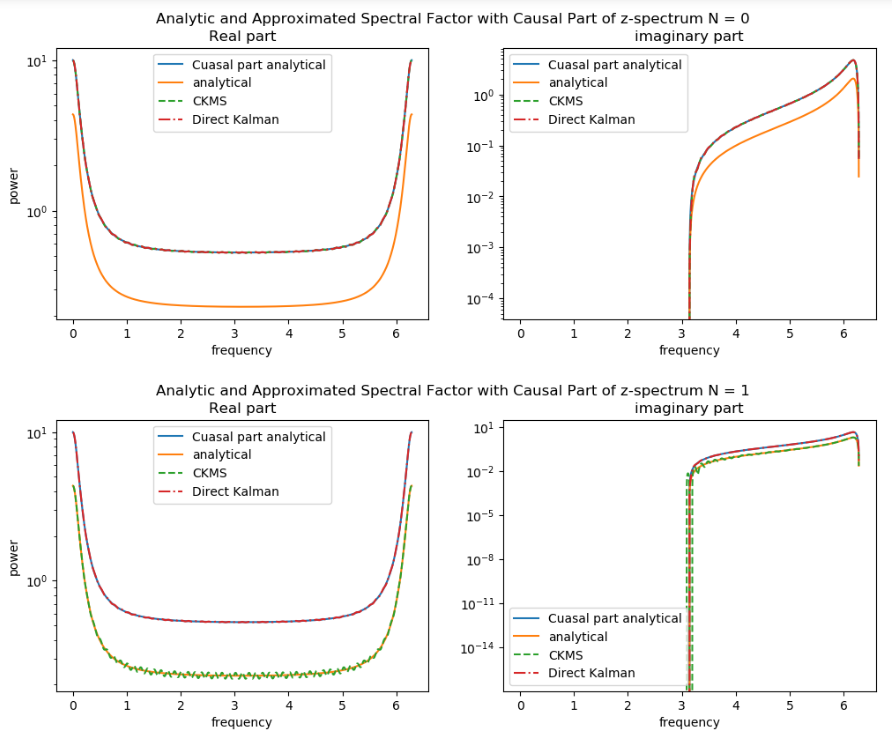
\includegraphics[scale=.8]{Example1N=0and1.png}
	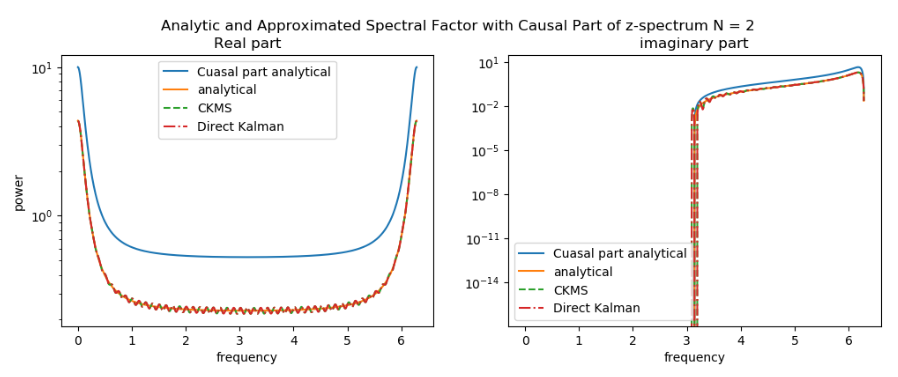
\includegraphics[scale=.8]{Example1N=2.png}
\end{figure}




\appendix

\section{CKMS}

CKMS, named for Chandrasekhar, Kailath, Morf, and Sidhu who in various ways and times contributed to its development, is an efficient algorithm for computing the Kalman filter recursion for innovations. I describe this briefly now. Kailath, Morf and Sidhu (1973) observed that though $P_i$ is full rank the change for one step to the next $\delta P_i := P_{i+1} - P_i$ can have low rank. So write,
	$$\delta P_i = L_iM_iL_i^*$$
It can be shown that if $\delta P_0 = L_0M_0L_0^*$ with $M_0$ hermitian, nonsingular, and of size $\alpha\times \alpha$, then for $i>0$, $\delta P_i = L_iM_iL_i^*$ with $M_i$ also hermitian, nonsingular, and of size $\alpha\times \alpha$. Exploiting this fact Kailath et al. provided the following theorem \cite[p.~409]{sayed2001}.
\begin{theorem}[The Fast (CKMS) Kalman Recursions ]
	The $K_{i}$ and $R_{e,i}$ from the Kalman recursion above can be recursively computed by the following set of coupled recursions, for $i\ge 0$
	\begin{align*}
	K_{i+1} &= K_{i} - FL_iR_{r,i}^{-1}L_i^*H^* \\
	L_{i+1} &= FL_{i} - K_{i}R_{e,i}^{-1}HL_i \\
	R_{e,i+1} &= R_{e,i} - HL_iR_{r,i}^{-1}L_i^*H^* \\
	R_{r,i+1} &= R_{r,i} - L_i^*H^*R_{e,i}^{-1}HL_i
	\end{align*}
	The recursion is initialized as follows: $K_{0} = F\Pi_0H^* + GS$ and $R_{e,0} = R+H\Pi_0H^*$. Then factor get $L_0$ and  $R_{r,0}$
	$$\delta P_0 := F\Pi_0F^* + GQG^* - K_{0}R_{e,0}^{-1}K_{0}^* - \Pi_0=:-L_0R_{r,0}^{-1}L_0^*$$ where $L_0$ is $m \times \alpha$ and $R_{r,0}$ is $\alpha \times \alpha$, nonsingular and Hermitian. 
\end{theorem}

An implementation of this method is summarized in Algorithm \ref{alg: CKMS}.
\begin{algorithm}
	\caption{Spectral Factorization by CKMS}
	\label{alg: CKMS}
	\begin{algorithmic}[1]
		\Procedure{KalmanSpecFac}{$C_\text{win}[0],C_\text{win}[1],\dots,
			C_\text{win}[m]$}
		\item[]
		\item[] {\bf Initialize variables}
		\State $F \gets \begin{pmatrix} 0 & & & \\ I & 0 & & \\ &\ddots & \ddots & \\ & & I & 0\end{pmatrix}$ \algorithmiccomment{$\in \C^{dm\times dm}$ (use sparse array)}
		\State $H \gets \begin{pmatrix} 0 & \dots & 0 & I\end{pmatrix}$ \algorithmiccomment{$\in \C^{dm\times dm}$ (use sparse array)}
		\State $K \gets \text{col}\big(C_\text{win}[m-i],\; i=0,1,\dots, m-1\big)$ \algorithmiccomment{$\in \C^{dm\times d}$}
		\State $L\gets \text{col}\big(C_\text{win}[m-i],\; i=0,1,\dots, m-1\big)$ \algorithmiccomment{$\in \C^{dm\times d}$}
		\State $R_e \gets C_\text{win}[0]$ \algorithmiccomment{$\in \C^{d\times d}$} 
		\State $R_r \gets C_\text{win}[0]$ \algorithmiccomment{$\in \C^{d\times d}$} 
		\item[]
		\item[] {\bf Run CKMS recursion}
		\State Assign $N>0$
		\For {$i = 1$ to $N$}
		\State	$K_\text{new} \gets K - FLR_{r}^{-1}L^*H^*$
		\State  $L_\text{new} \gets FL - KR_e^{-1}hL$
		\State  $R_{e,\text{new}} \gets R_e - HLR_r^{-1}L^*H^*$
		\State  $R_{r,\text{new}} \gets R_r - L^*H^*R_e^{-1}HL$
		\item[]
		\State	$K \gets K_\text{new}$
		\State  $L \gets L_\text{new}$
		\State  $R_{e} \gets R_{e,\text{new}}$
		\State  $R_{r} \gets R_{r,\text{new}}$
		\EndFor
		\item[]
		\item[] {\bf Extract spectral factor coefficients}
		\State $K\gets K/R_e$
		\State $R_e \gets \sqrt{R_e}$
		\State $\ell \gets$ zeros($d,d,m+1$)
		\For{$i = 0$ to $m$}
		\State $\ell[:,:,m-i+1] \gets K[di + 1: d(i+1),:]R_e$
		\EndFor
		\Return $\ell$
		
		\EndProcedure
	\end{algorithmic}	
\end{algorithm}

\section{Proof of Lemma \ref{lem: otho p}}
\label{app: Ortho proof}
Lemma \ref{lem: otho p} has been restated for convenience.
\begin{lem}
	Given the inner product defined under (\ref{def: inner p}) and the norm induced by it, under (\ref{def: norm}), let $x\in C^d$ and $y_i \in \C^m$ for $i=0,\dots,N$ be random variables. If $\hat x\in \text{span}_d\{y_i,\;i=0,1\dots,N\}$ is chosen such that \begin{equation}
	(x-\hat x) \perp y_i \qquad\text{\emph{for}}\qquad i=0,1,\dots,N,
	\end{equation}
	then $\hat x$ is the linear LMSE for $x$ given $\{y_i,\;i=0,\dots,N\}$, meaning
	$$\E(x-\hat x)(x-\hat x)^* = \|x-\hat x\|^2 = \inf_{x'\in \text{\emph{span}}_d\{y_i,\;\forall i\}} \|x-x'\|^2.$$
\end{lem}
\begin{proof}
	Let $x' \in \text{span}_d\{y_i,\;\forall i\}$ and observe that since $\hat x - x' \in \text{span}_d\{y_i,\;\forall i\}$. The orthogonality assumption amounts to $x-\hat x$ being orthogonal to every element in $\text{span}_d\{y_i,\;\forall i\}$ and so $(x-\hat x) \perp (\hat x - x')$. Then we can write
	$$\|x-x'\|^2 = \|x-\hat x + \hat x - x'\|^2 = \|x-\hat x \|^2 + \|\hat x - x'\|^2 \ge \|x-\hat x \|^2$$
	which completes the proof.
\end{proof}




\section{Illustration}
Consider this iterative algorithm for finding the square root of a positive number $x$. 

\begin{algorithm}
	\caption{Square Root (Analogue of CKMS)}
	\label{alg: sqrt CKMS}
	\begin{algorithmic}[1]
		\Procedure{mysqrt1}{$x$}
		\State $x_0 \gets x$
		\State Assign $N>0$
		\For {$i = 1$ to $N$}
		\State	$x \gets \dfrac{1}{2}\left(x+\dfrac{x_0}{x}\right)$
		\EndFor
		\item[]
		\Return $x$		
		\EndProcedure
	\end{algorithmic}	
\end{algorithm}

\begin{algorithm}
	\caption{Square Root (Analogue of Direct Kalman)}
	\label{alg: sqrt Kalman}
	\begin{algorithmic}[1]
		\Procedure{mysqrt2}{$x$}
		\State $x_0 \gets x$
		\State $x \gets 1$
		\State Assign $N>0$
		\For {$i = 1$ to $N$}
		\State	$x \gets \dfrac{1}{2}\left(x+\dfrac{x_0}{x}\right)$
		\EndFor
		\item[]
		\Return $x$		
		\EndProcedure
	\end{algorithmic}	
\end{algorithm}

\bibliographystyle{unsrt}
\bibliography{../Notes}
\end{document}
